\documentclass[aspectratio=169,11pt]{beamer}
\usepackage[T1]{fontenc}
\usepackage[utf8]{inputenc}
\usepackage{lmodern}
\usepackage{amsmath,amssymb,booktabs,graphicx,xcolor,ragged2e,tikz}
\usepackage{hyperref}
\hypersetup{colorlinks=true,urlcolor=blue}
\graphicspath{{../pilot/run_corrected/}}

% A restrained academic palette: navy + teal + amber.
\definecolor{Navy}{HTML}{12304A}
\definecolor{Teal}{HTML}{007C83}
\definecolor{Amber}{HTML}{D98E04}
\definecolor{Ink}{HTML}{1B2630}
\definecolor{Mist}{HTML}{F3F6F8}
\definecolor{Muted}{HTML}{5B6B75}

\setbeamercolor{normal text}{fg=Ink,bg=white}
\setbeamercolor{structure}{fg=Navy}
\setbeamercolor{frametitle}{fg=Navy,bg=white}
\setbeamercolor{title}{fg=white}
\setbeamercolor{subtitle}{fg=white!85!Navy}
\setbeamercolor{block title}{fg=white,bg=Navy}
\setbeamercolor{block body}{fg=Ink,bg=Mist}
\setbeamercolor{alerted text}{fg=Amber}
\setbeamertemplate{navigation symbols}{}
\setbeamertemplate{frametitle}{%
  \vspace{0.25cm}\hspace{0.15cm}\insertframetitle\par\vspace{0.08cm}%
  \hspace{0.15cm}\color{Teal}\rule{\dimexpr\paperwidth-0.3cm\relax}{1.2pt}}
\setbeamertemplate{footline}{%
  \leavevmode\hbox{\begin{beamercolorbox}[wd=.78\paperwidth,ht=2.6ex,dp=1.1ex,leftskip=.25cm]{author in head/foot}\color{Muted}\scriptsize MTP progress presentation\end{beamercolorbox}%
  \begin{beamercolorbox}[wd=.22\paperwidth,ht=2.6ex,dp=1.1ex,rightskip=.25cm plus1fil]{date in head/foot}\color{Muted}\scriptsize\insertframenumber/\inserttotalframenumber\end{beamercolorbox}}}
\setbeamertemplate{itemize item}{\color{Teal}\small\raisebox{0.2ex}{\textbullet}}
\setbeamertemplate{itemize subitem}{\color{Amber}\scriptsize\raisebox{0.2ex}{\textbullet}}
\setlength{\leftmargini}{1.2em}

\title{Artifact-Aware Stability of Fractal Features\\in Depth-Indexed Well Logs}
\subtitle{Corrected fBm/fGn generator and bounded FORCE 2020 pilot}
\author{Master's Thesis Project (MTP)}
\institute{Research progress presentation for the research guide}
\date{24 September 2026}

\begin{document}

{\setbeamertemplate{footline}{}
\begin{frame}[plain]
\begin{tikzpicture}[remember picture,overlay]
  \fill[Navy] (current page.south west) rectangle (current page.north east);
  \fill[Teal] (current page.south west) rectangle ([xshift=.22\paperwidth]current page.north west);
  \fill[Amber] ([xshift=.22\paperwidth]current page.south west) rectangle ([xshift=.235\paperwidth]current page.north west);
\end{tikzpicture}
\vspace{0.7cm}
\hspace{0.35cm}\begin{minipage}{0.87\textwidth}
{\color{white}\fontsize{25}{30}\selectfont\bfseries Artifact-Aware Stability of Fractal Features\\[0.12cm]in Depth-Indexed Well Logs\par}
\vspace{0.55cm}
{\color{white!85!Navy}\Large Corrected fBm/fGn generator and bounded FORCE 2020 pilot\par}
\vfill
{\color{white}\large Master's Thesis Project (MTP)\par}
\vspace{0.15cm}
{\color{white!80!Navy}\normalsize Research progress presentation for the research guide\\24 September 2026\par}
\end{minipage}
\end{frame}}

\begin{frame}{The one-sentence message}
\begin{center}
\vspace{0.35cm}
\begin{beamercolorbox}[sep=0.5cm,wd=.9\textwidth]{block body}
\centering\Large\bfseries
The corrected generator recovers known synthetic H values,\\[0.15cm]
but real GR intervals do not support one stable,\\[0.15cm]
unqualified H estimate across estimators.
\end{beamercolorbox}
\vspace{0.55cm}
\normalsize
This is a methodological result: \alert{validate the physical scale and estimator before geological interpretation.}
\end{center}
\end{frame}

\begin{frame}{Why this problem matters}
\begin{columns}[T,onlytextwidth]
\column{.47\textwidth}
\textcolor{Navy}{\Large\bfseries Fractal attributes are attractive}
\vspace{0.2cm}
\begin{itemize}
  \item Compact summaries of roughness and scaling
  \item Used in well-log and reservoir studies
  \item Potentially useful for multiscale heterogeneity
\end{itemize}
\column{.47\textwidth}
\textcolor{Amber}{\Large\bfseries But measurements can move}
\vspace{0.2cm}
\begin{itemize}
  \item Sampling interval and filtering alter scales
  \item Finite records limit the fit range
  \item Geological regime mixing can mimic scaling
\end{itemize}
\end{columns}
\vfill
\begin{beamercolorbox}[sep=0.25cm,wd=\textwidth]{block body}
\centering\textbf{Research need:} distinguish genuine signal structure from acquisition and analysis artifacts.
\end{beamercolorbox}
\end{frame}

\begin{frame}{Research question and contribution}
\begin{beamercolorbox}[sep=0.35cm,wd=\textwidth]{block body}
\large\textbf{Question}\par\vspace{0.1cm}
Under controlled sampling and filtering perturbations, which established fractal features extracted from depth-indexed well logs are recoverable, stable, and interpretable over a declared physical scale range?
\end{beamercolorbox}
\vspace{0.35cm}
\textcolor{Teal}{\Large\bfseries Proposed contribution}
\begin{itemize}
  \item Not a new estimator
  \item A reproducible artifact-aware stability benchmark
  \item Known-answer synthetic validation before real-log interpretation
  \item Transparent no-go outcomes when estimators disagree
\end{itemize}
\end{frame}

\begin{frame}{Where the MTP has reached}
\begin{columns}[T,onlytextwidth]
\column{.48\textwidth}
\textcolor{Teal}{\Large\bfseries Completed}
\begin{itemize}
  \item Literature inventory and scoped review
  \item 40 research ideas screened
  \item Primary direction selected
  \item FORCE 2020 dataset audited
  \item Corrected generator implemented
  \item 4 automated tests passing
\end{itemize}
\column{.48\textwidth}
\textcolor{Amber}{\Large\bfseries Current decision point}
\begin{itemize}
  \item Synthetic recovery: pass
  \item Real stable-single-H interpretation: no-go
  \item Monofractal protocol needs broader calibration
  \item Multifractal extension remains deferred
\end{itemize}
\end{columns}
\end{frame}

\begin{frame}{Corrected stochastic construction}
\begin{columns}[T,onlytextwidth]
\column{.54\textwidth}
\small
For $0<H<1$, the stationary fGn covariance is
\begin{equation*}
C_H(k)=\frac{1}{2}\left[(k+1)^{2H}-2k^{2H}+|k-1|^{2H}\right].
\end{equation*}
\vspace{0.15cm}
\begin{enumerate}
  \item Build the circulant covariance embedding
  \item Check Fourier eigenvalues for positive semidefiniteness
  \item Generate Gaussian fGn increments $G_i$
  \item Form fBm-like levels: $B_j=\sum_{i<j}G_i$
\end{enumerate}
\column{.42\textwidth}
\begin{beamercolorbox}[sep=0.3cm,wd=\textwidth]{block body}
\centering
{\textcolor{Navy}{\Large Key distinction}}\\[0.15cm]
\textbf{fGn:} stationary increments; \textbf{fBm levels:} nonstationary, stationary increments
\end{beamercolorbox}
\vspace{0.3cm}
\centering\textcolor{Teal}{\large No silent eigenvalue clipping}
\end{columns}
\end{frame}

\begin{frame}{Bounded experimental design}
\begin{columns}[T,onlytextwidth]
\column{.5\textwidth}
\textcolor{Navy}{\Large\bfseries Synthetic controls}
\begin{itemize}
  \item $H\in\{0.2,0.5,0.8\}$
  \item Four fixed seeds per H
  \item 8192 fGn increments per realization
  \item Variogram on levels
  \item Spectrum on first differences
\end{itemize}
\column{.5\textwidth}
\textcolor{Navy}{\Large\bfseries Real GR pilot}
\begin{itemize}
  \item FORCE 2020 LAS wells
  \item Contiguous finite uniform blocks
  \item 4097 points per selected interval
  \item Baseline, smoothing, downsample $\times2$, $\times4$
  \item Common physical lag/frequency bands
\end{itemize}
\end{columns}
\vfill
\begin{beamercolorbox}[sep=0.22cm,wd=\textwidth]{block body}
\centering\small No interpolation across gaps; no post-hoc tuning of seeds, thresholds, or scales.
\end{beamercolorbox}
\end{frame}

\begin{frame}{Synthetic recovery: the implementation works}
\begin{table}
\centering\small
\begin{tabular}{@{}ccrrc@{}}
\toprule
Known $H$ & Estimator & Bias & RMSE & Gate\\
\midrule
0.2 & Variogram & -0.0135 & 0.0270 & Pass\\
0.2 & Spectral & -0.0143 & 0.0653 & Pass\\
0.5 & Variogram & -0.0199 & 0.0333 & Pass\\
0.5 & Spectral &  0.0051 & 0.0637 & Pass\\
0.8 & Variogram & -0.0285 & 0.0463 & Pass\\
0.8 & Spectral &  0.0068 & 0.0637 & Pass\\
\bottomrule
\end{tabular}
\end{table}
\vspace{0.2cm}
\begin{center}
\textcolor{Teal}{\Large\bfseries Known-answer synthetic gate: PASS}\par
\small The covariance-based generator and estimator conventions are internally consistent for this bounded test.
\end{center}
\end{frame}

\begin{frame}{Synthetic estimates across known H values}
\centering
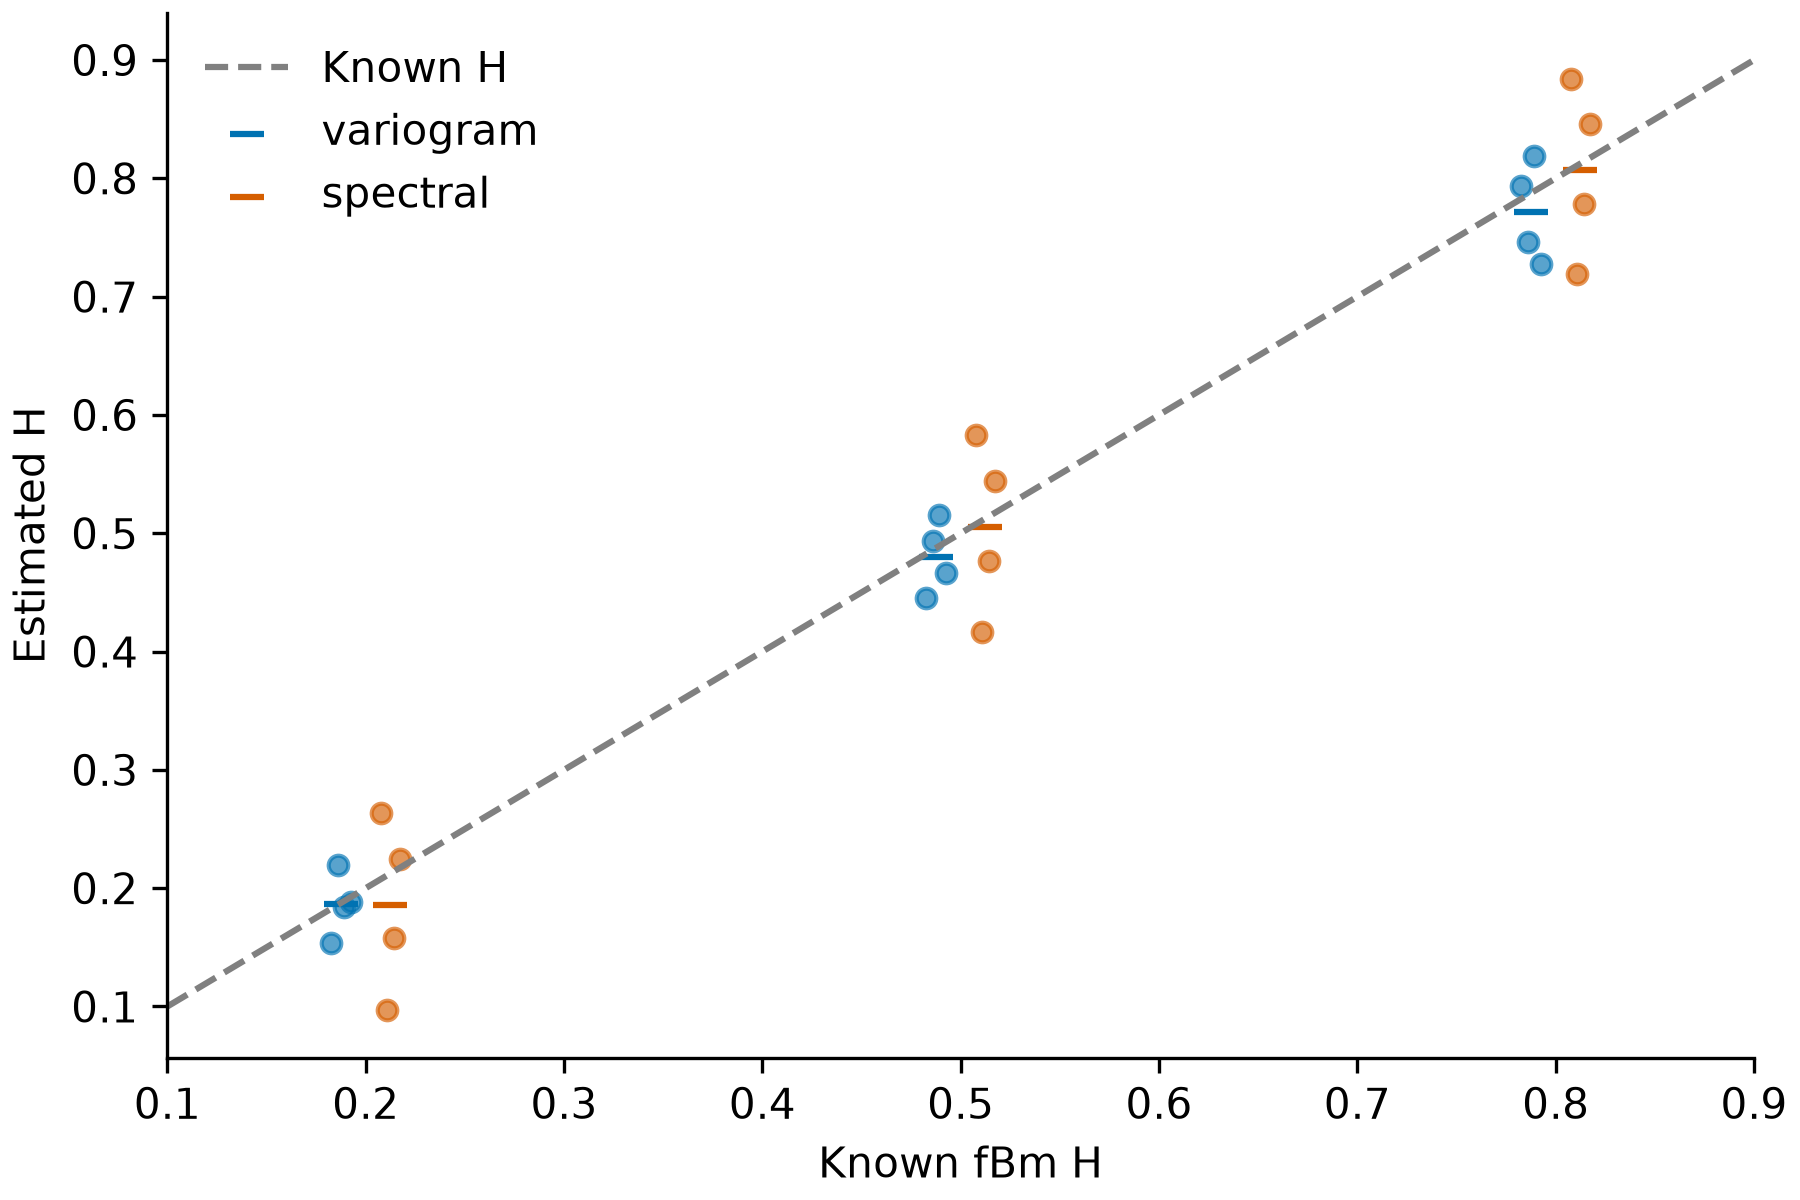
\includegraphics[width=.91\textwidth,height=.71\textheight,keepaspectratio]{Figure_1.png}
\vspace{-0.1cm}
\scriptsize Individual seeds and estimator summaries from the executed pilot.
\end{frame}

\begin{frame}{Real GR pilot: estimator disagreement is the finding}
\begin{table}
\centering\small
\begin{tabular}{@{}lrrrr@{}}
\toprule
Well & Variogram H & Spectral H & Largest $|\Delta H|$ & Gate\\
\midrule
15\_9-13 & 0.3867 & -0.1087 & 0.0945 & Fail\\
15\_9-14 & 0.3382 &  0.1143 & 0.0944 & Fail\\
15\_9-15 & 0.3050 &  0.0163 & 0.0946 & Fail\\
\bottomrule
\end{tabular}
\end{table}
\vspace{0.25cm}
\begin{beamercolorbox}[sep=0.28cm,wd=\textwidth]{block body}
\centering\textbf{Interpretation:} perturbation changes were modest, but baseline estimator disagreement exceeded the stability criterion.
\end{beamercolorbox}
\end{frame}

\begin{frame}{Real-log sensitivity under controlled perturbations}
\centering
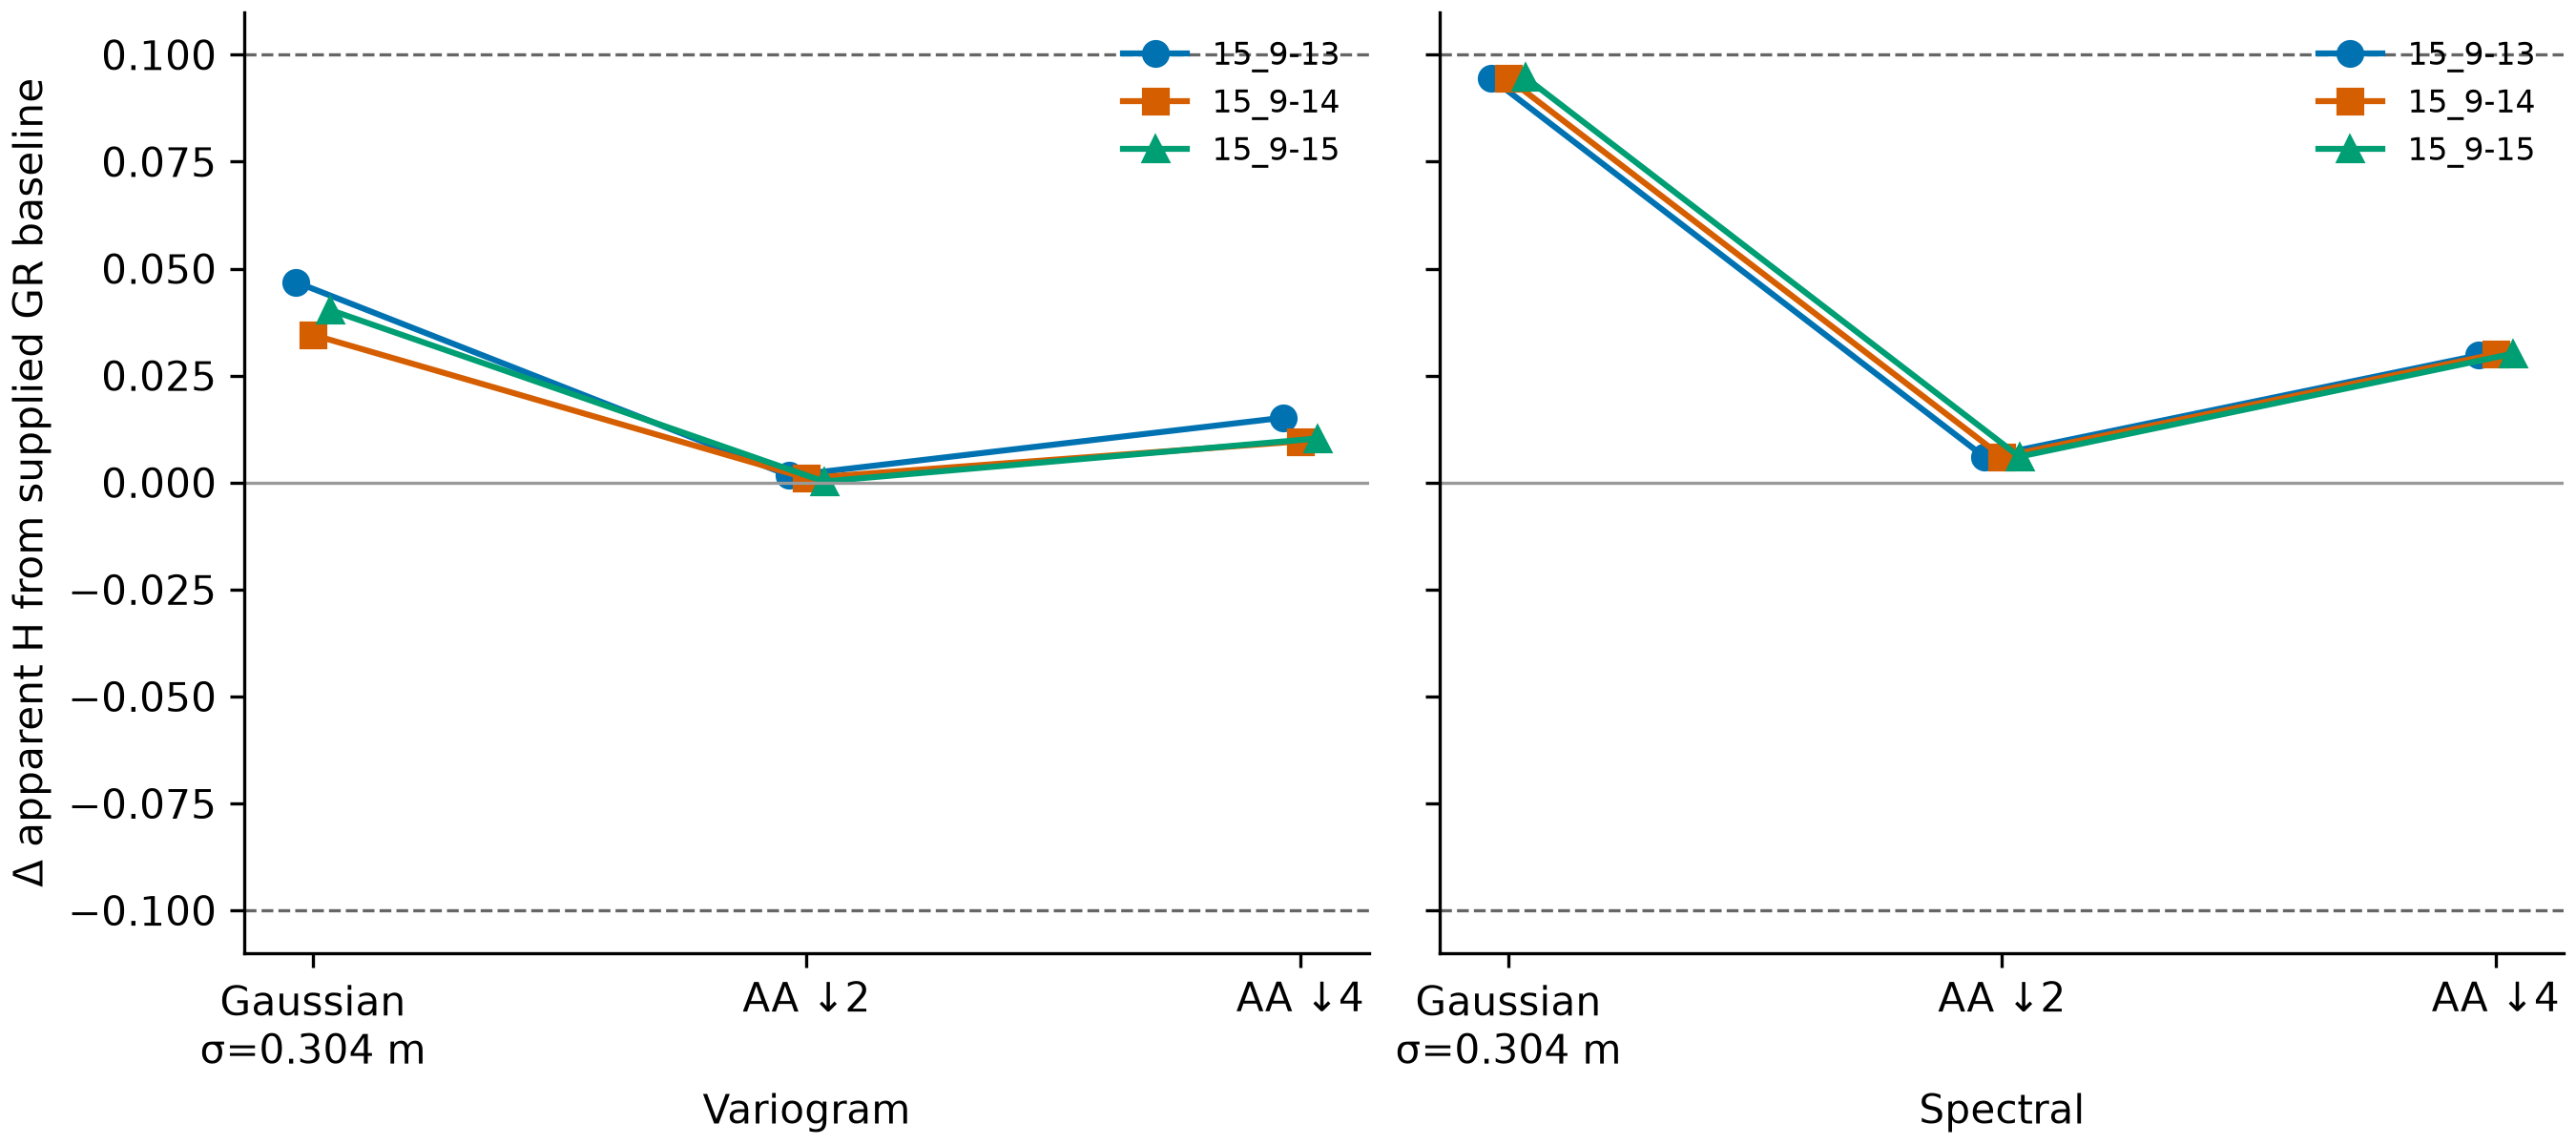
\includegraphics[width=.91\textwidth,height=.73\textheight,keepaspectratio]{Figure_2.png}
\vspace{-0.1cm}
\scriptsize Changes are relative to each interval's baseline; they are descriptive, not geological accuracy estimates.
\end{frame}

\begin{frame}{What the no-go means}
\begin{columns}[T,onlytextwidth]
\column{.48\textwidth}
\textcolor{Amber}{\Large\bfseries It does mean}
\begin{itemize}
  \item Do not report one universal H for these intervals
  \item Estimator agreement is not automatic
  \item Physical fit bands must be declared
  \item Real-log conclusions require sensitivity reporting
\end{itemize}
\column{.48\textwidth}
\textcolor{Teal}{\Large\bfseries It does not mean}
\begin{itemize}
  \item The generator failed
  \item The logs contain no scaling structure
  \item One estimator is universally correct
  \item The broader MTP is invalid
\end{itemize}
\end{columns}
\end{frame}

\begin{frame}{Limitations and next steps}
\textcolor{Navy}{\Large\bfseries Immediate next steps}
\begin{enumerate}
  \item Increase synthetic calibration to at least 30 realizations per H
  \item Report Monte Carlo uncertainty and failure fractions
  \item Freeze physical bands before the next real-log analysis
  \item Add predetermined geological-context windows and rejection ledger
  \item Test measured or defensible tool-response filters
\end{enumerate}
\vspace{0.2cm}
\begin{beamercolorbox}[sep=0.25cm,wd=\textwidth]{block body}
\textbf{Only after monofractal calibration:} consider a measure-specific multifractal and surrogate-control extension.
\end{beamercolorbox}
\end{frame}

\begin{frame}{Conclusion}
\begin{enumerate}
  \item The corrected fBm/fGn generator is implemented and verified.
  \item Synthetic known-answer recovery passes the bounded gate.
  \item Three real GR intervals fail the stable single-H interpretation criterion.
  \item The scientifically defensible contribution is an artifact-aware validation protocol.
\end{enumerate}
\vfill
\begin{beamercolorbox}[sep=0.35cm,wd=\textwidth]{block body}
\centering\Large\bfseries Next decision: approve the expanded monofractal calibration stage.
\end{beamercolorbox}
\end{frame}

\begin{frame}[plain]
\begin{center}
\vfill
{\color{Navy}\fontsize{30}{34}\selectfont\bfseries Thank you}\par
\vspace{0.35cm}
{\color{Teal}\Large Questions and guidance}\par
\vfill
\small
Code, tests, report, figures, and JSON results are archived in the MTP project directory.
\end{center}
\end{frame}

\end{document}
